\documentclass[10pt,twocolumn]{article}
\usepackage[margin=0.9in]{geometry}
\usepackage{graphicx,booktabs,amsmath}
\usepackage{caption}
\usepackage{subcaption}
\graphicspath{{figures/}}
\begin{document}

% ---- Variant 1: one combined figure spanning both columns ----
\begin{figure*}[t]
  \centering
  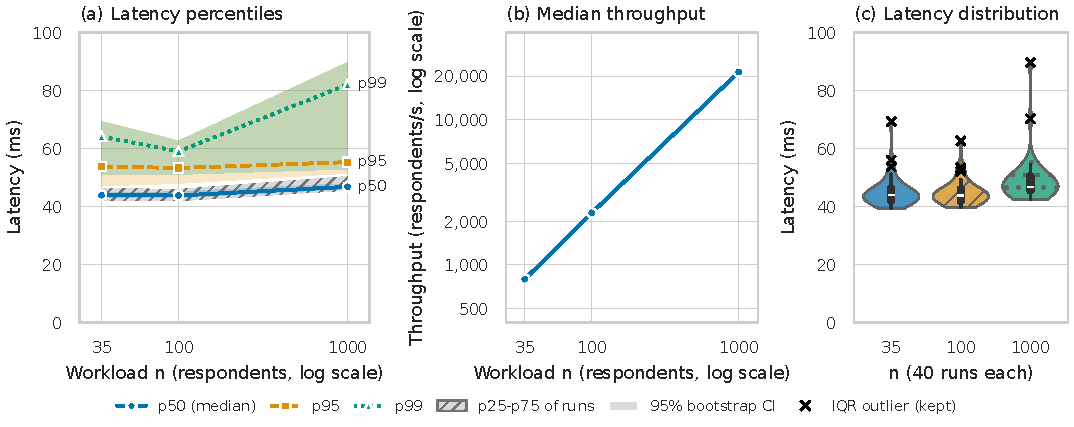
\includegraphics[width=\textwidth]{fig_combined_latency_throughput.pdf}
  \caption{Latency and throughput of the survey-processing pipeline for workloads of
  $n=35$, $100$ and $1000$ respondents (40 runs per size, $N=120$). \textbf{(a)}~Latency
  percentiles p50, p95 and p99; coloured bands are 95\% percentile-bootstrap confidence
  intervals ($B=10{,}000$, seed 42), the grey hatched band is the interquartile range
  (p25--p75) of the per-run latencies. \textbf{(b)}~Median throughput on log--log axes; the
  band is the 95\% bootstrap CI. \textbf{(c)}~Distribution of per-run latency; the inner box
  shows p25, p50 and p75, crosses mark IQR-rule outliers (9 of 120), which were kept in
  all statistics. Median latency rises only from 43.9\,ms to 46.8\,ms while throughput grows
  from 797 to 21\,371 respondents/s ($\times 26.8$ for a $\times 28.6$ larger workload).}
  \label{fig:combined}
\end{figure*}

% ---- Variant 2: three separate panels with subcaption ----
\begin{figure*}[t]
  \centering
  \begin{subfigure}[t]{0.34\textwidth}
    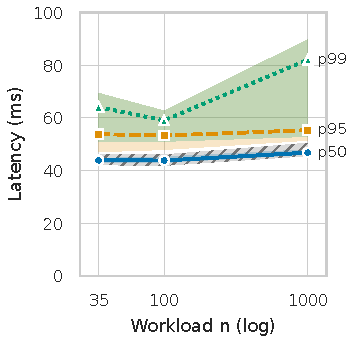
\includegraphics[width=\linewidth]{fig_panel_a.pdf}
    \caption{Latency percentiles with 95\% CI bands.}\label{fig:panel-a}
  \end{subfigure}\hfill
  \begin{subfigure}[t]{0.32\textwidth}
    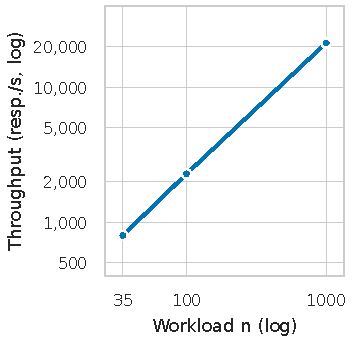
\includegraphics[width=\linewidth]{fig_panel_b.pdf}
    \caption{Median throughput (log--log).}\label{fig:panel-b}
  \end{subfigure}\hfill
  \begin{subfigure}[t]{0.30\textwidth}
    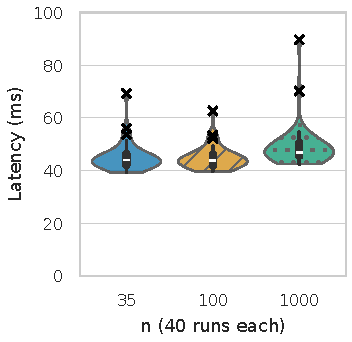
\includegraphics[width=\linewidth]{fig_panel_c.pdf}
    \caption{Per-run latency distribution.}\label{fig:panel-c}
  \end{subfigure}
  \caption{Same data as Fig.~\ref{fig:combined}, panels placed separately. Panel~(\subref{fig:panel-a})
  shows p50/p95/p99 with 95\% bootstrap CIs; Panel~(\subref{fig:panel-b}) the median throughput;
  Panel~(\subref{fig:panel-c}) the 40 per-run latencies per workload, crosses = IQR outliers (kept).}
  \label{fig:split}
\end{figure*}

Text referring to Fig.~\ref{fig:combined}, \ref{fig:panel-a}.
\end{document}
